\section{Benchmark}

\begin{figure}[t]
\centering
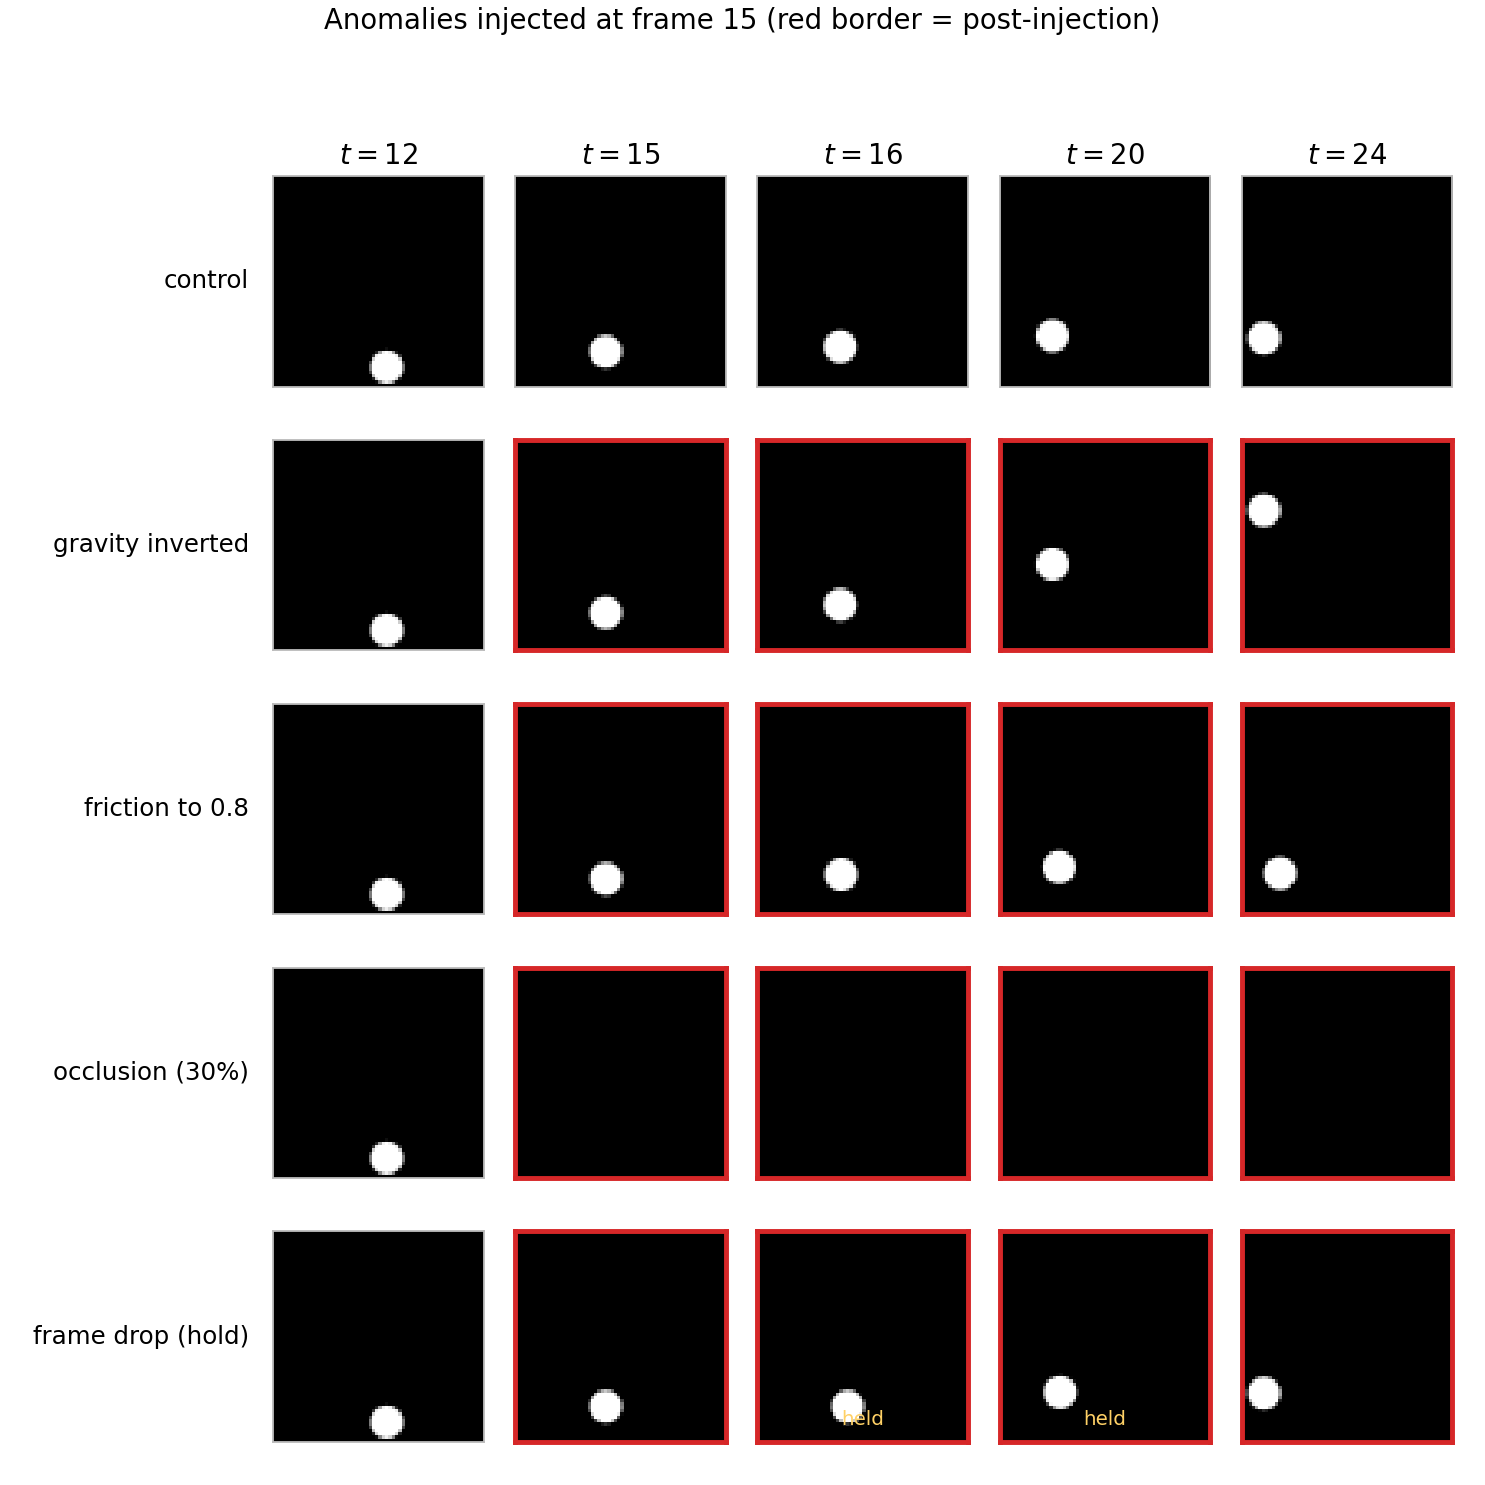
\includegraphics[width=0.86\linewidth]{generated/fig_dataset.png}
\caption{The four anomaly families, one row each, against the control row. Red
borders mark post-injection frames; ``held'' marks a frame the sensor glitch
repeats. All conditions share the control's pre-injection history exactly, so
every comparison is paired at the clip level.}
\label{fig:dataset}
\end{figure}

A disc of radius $5$ bounces inside a $64\times64$ frame for $30$ frames under
constant downward gravity $g_0 = 0.25\,\mathrm{px/frame^2}$ with perfectly
elastic collisions, so the baseline dynamics conserve energy and are
statistically stationary. Initial position, speed and direction are randomised;
generation is deterministic given the frozen seed.

At frame $t^\star=15$ one of four anomalies is injected
(Figure~\ref{fig:dataset}):

\begin{description}
\item[gravity inverted] $g \to -g_0$. Acceleration changes immediately;
position diverges only gradually, which makes this the subtlest condition at
short latency.
\item[friction] per-frame velocity retention $0.8^{1/5}$ and bounce restitution
$0.8$. Applied per frame rather than only at collisions, so the effect is
observable from the first post-injection frame; a collision-only version would
leave time-to-alarm undefined on clips with no bounce in the window.
\item[occlusion] a static black square of $29.9\%$ frame area, anchored on the
disc's path.
\item[frame drop] for underlying frames $15..22$, every other frame is not
delivered and the previous frame is held in its place --- four held frames ---
with normal delivery resuming at frame $23$.
\end{description}

\paragraph{What the occlusion condition actually tests.}
A $35\times35$ square anchored on the trajectory of a $10$-pixel disc does not
``partially block'' it. Measured across the condition,
\lgwOccFullyHidden{} of post-injection frames hide the disc completely,
\lgwOccPartial{} hide it partially, and in \lgwOccFullyHiddenClips{} of clips
the disc is never visible again inside the window. This condition therefore
probes object permanence --- does the representation register that a tracked
object has vanished --- rather than robustness to partial visual corruption. We
report it as such. It follows directly from the registered specification and is
not a defect, but describing it as partial occlusion would misstate what the
numbers mean.

\paragraph{Effect sizes are not comparable across conditions.}
Gravity inversion changes acceleration at once; friction changes velocity by
about $4.4\%$ per frame; occlusion removes the object; the frame drop freezes
it. These are different magnitudes of disturbance, so pooled results average
over heterogeneous effects, and per-condition results are reported separately.

\paragraph{Paired design.}
An anomalous clip and its control share a random seed, so their frames are
identical up to $t^\star$ and diverge only because of the injection. Every
monitor comparison is therefore within-clip, which is what the paired tests in
Section~\ref{sec:protocol} exploit.

\paragraph{Scale.}
The registered design is $1000$ anomalous clips ($250$ per condition) plus $200$
controls split into $\lgwNCalib$ calibration and $\lgwNEval$ evaluation. Clips
are bilinearly upsampled to the model's native resolution and replicated to
three channels.
